\documentclass[conference,letterpaper,10pt]{IEEEtran}
\usepackage[T1]{fontenc}
\usepackage[utf8]{inputenc}
\usepackage[spanish,es-tabla,es-nodecimaldot]{babel}
\usepackage{times,graphicx,booktabs,amsmath,amssymb,url,tabularx,array}
\usepackage[numbers]{natbib}
\newcommand{\rdias}{121}
\newcommand{\recoEF}{102,135}
\newcommand{\recoE}{84,956}
\newcommand{\recoF}{17,178}
\newcommand{\rbaseEF}{220,061}
\newcommand{\rbaseE}{169,276}
\newcommand{\rbaseF}{50,785}
\newcommand{\rmaEF}{57,802}
\newcommand{\rmaE}{53,774}
\newcommand{\rmaF}{4,028}
\newcommand{\recoVis}{2,263}
\newcommand{\recoBicis}{10,276}
\newcommand{\rmaVis}{2,060}
\newcommand{\rmaBicis}{10,084}
\newcommand{\rmaPct}{43.4}
\newcommand{\rmaPctLo}{41.2}
\newcommand{\rmaPctHi}{45.6}
\newcommand{\rlgbmDPct}{43.0}
\newcommand{\rlgbmDEF}{58,187}
\newcommand{\rlgbmDirPct}{43.7}
\newcommand{\rlgbmDirEF}{57,510}
\newcommand{\rorDPct}{60.0}
\newcommand{\rorDEF}{40,872}
\newcommand{\rorDirPct}{67.0}
\newcommand{\rorDirEF}{33,684}
\newcommand{\rmaGana}{121}
\newcommand{\rmaVisPct}{9.0}
\newcommand{\rmaGap}{16,930}
\newcommand{\rlgbmDirGap}{23,826}
\newcommand{\roracleDirectGap}{7,187}
\newcommand{\rmaDesvSal}{3,395}
\newcommand{\rmaDesvLleg}{311}
\newcommand{\rmaKm}{0.25}
\newcommand{\recoDesv}{2,298}
\newcommand{\recoKm}{0.26}
\newcommand{\recoNeto}{51.3}
\newcommand{\rdicPct}{39.2}
\newcommand{\rdicDias}{31}
\newcommand{\rdicMes}{diciembre de 2025}
\newcommand{\rdecTot}{44,770}
\newcommand{\rdecPNoventaCinco}{0.1}
\newcommand{\rnDiario}{4}
\newcommand{\rnDirecto}{4}
\newcommand{\rselDias}{31}
\newcommand{\rlamMa}{58.2}
\newcommand{\rlamLgbmD}{59.2}
\newcommand{\rlamLgbmDir}{68.9}
\newcommand{\rlamOrD}{44.6}
\newcommand{\rlamOrDir}{36.3}
\newcommand{\rlamDifMax}{0.89}
\newcommand{\rlamRondasMax}{4}
\newcommand{\rlamExtension}{0}
\newcommand{\rlamGridMin}{10}
\newcommand{\rlamGridMax}{120}
\newcommand{\rlamGrid}{10, 15, 20, 30, 45, 60, 75, 90, 120}
\newcommand{\rmejorReal}{media móvil}
\newcommand{\rselEcoVis}{2,033.9}
\newcommand{\rselMaVis}{2,051.5}
\newcommand{\rtopeVis}{55}
\newcommand{\rtopeBicis}{17}
\newcommand{\rpickMin}{15}
\newcommand{\rdelMin}{60}
\newcommand{\rstepMin}{15}
\newcommand{\rlagS}{30}
\newcommand{\rcovMin}{90}
\newcommand{\rtransMin}{45}
\newcommand{\rentregaCorta}{45}
\newcommand{\rentregaLarga}{75}
\newcommand{\rventanaHoras}{19.5}
\newcommand{\rabiertaPct}{95}
\newcommand{\rrefDias}{15}
\newcommand{\rnMax}{6}
\newcommand{\rlamGridN}{15, 30, 60}
\newcommand{\rtrainMeses}{8}
\newcommand{\rcurvaDias}{121}
\newcommand{\rsemanasHist}{4}
\newcommand{\rcadaTicks}{12}
\newcommand{\rlgbArboles}{200}
\newcommand{\rlgbTasa}{0.05}
\newcommand{\rlgbHojas}{31}
\newcommand{\rlgbMinHoja}{50}
\newcommand{\rlgbFilas}{0.8}
\newcommand{\rlgbCols}{0.9}
\newcommand{\rviajes}{18,689,701}
\newcommand{\rdatosPeriodo}{enero y noviembre de 2025}
\newcommand{\rviajesDia}{55,957}
\newcommand{\restaciones}{677}
\newcommand{\rbicisDistintas}{7,966}
\newcommand{\rdurMed}{12}
\newcommand{\rdurP}{37}
\newcommand{\rhuecoMed}{15.9}
\newcommand{\rhuecoTarde}{35.6}
\newcommand{\rhuecoResto}{15.3}
\newcommand{\rcalleMed}{5.3}
\newcommand{\rpicoMed}{24}
\newcommand{\rpicoNoventa}{44}
\newcommand{\rpicoNN}{61}
\newcommand{\rvDias}{121}
\newcommand{\rvEobs}{87,470}
\newcommand{\rvFobs}{17,062}
\newcommand{\rvErep}{84,956}
\newcommand{\rvFrep}{17,178}
\newcommand{\rvRel}{3}
\newcommand{\rvRelF}{-1}
\newcommand{\rsCuarenta}{$-$6,559}
\newcommand{\rsCuarentaLo}{$-$7,042}
\newcommand{\rsCuarentaHi}{$-$6,076}
\newcommand{\rsCuarentaOr}{$-$3,906}
\newcommand{\rsSetenta}{$+$6,922}
\newcommand{\rsSetentaLo}{$+$6,348}
\newcommand{\rsSetentaHi}{$+$7,496}
\newcommand{\rsSetentaOr}{$+$3,476}
\newcommand{\rsDan}{$+$1,253}
\newcommand{\rsDanLo}{$+$952}
\newcommand{\rsDanHi}{$+$1,554}
\newcommand{\rsDanOr}{$+$89}
\newcommand{\rsSinRegla}{4,615}
\newcommand{\rsSoloUno}{2,470}
\newcommand{\rsEcoEF}{102,135}
\newcommand{\rmaeMes}{septiembre de 2025}
\newcommand{\rmaeMa}{1.62}
\newcommand{\rmaeMaW}{0.81}
\newcommand{\rmaeLgbmD}{1.61}
\newcommand{\rmaeLgbmDW}{0.81}
\newcommand{\rmaeLgbmDir}{1.99}
\newcommand{\rmaeLgbmDirW}{0.88}
\newcommand{\rantPeriodo}{enero a agosto de 2025}
\newcommand{\rvisSinRegla}{5,113.5}
\newcommand{\rvisConRegla}{2,491.5}
\newcommand{\rvisQuedan}{48.7}
\newcommand{\rpruebaPeriodo}{septiembre a diciembre de 2025}
\newcommand{\rselMes}{agosto de 2025}
\newcommand{\rrefPeriodo}{septiembre a noviembre de 2025}
\newcommand{\retiquetasDia}{5,000}
\newcommand{\renSitioPct}{78}
\newcommand{\rfdFeedE}{87,470}
\newcommand{\rfdFeedF}{17,062}
\newcommand{\rfdFeedEF}{104,532}
\newcommand{\rfdSalidasDia}{52,243}
\newcommand{\recoDesvPct}{4.4}
\newcommand{\rmaDesvPct}{7.1}
\newcommand{\rorDirDesvPct}{3.6}
\newcommand{\rlgbmDirDesvPct}{7.5}
\newcommand{\rbaseDesvPct}{27.0}
\newcommand{\rfdEcoDesv}{2,298}
\newcommand{\rcfDias}{16}
\newcommand{\rcfPrimero}{1 de septiembre de 2025}
\newcommand{\rcfUltimo}{31 de diciembre de 2025}
\newcommand{\rcfSalidas}{856,176}
\newcommand{\rcfEcoDesv}{38,825}
\newcommand{\rcfEcoPct}{4.53}
\newcommand{\rcUnoSal}{22}
\newcommand{\rcUnoLle}{35}
\newcommand{\rcUnoTSal}{4.6}
\newcommand{\rcUnoTLle}{5.3}
\newcommand{\rcDosPct}{5.2}
\newcommand{\rcDosMin}{1.3}
\newcommand{\rcDosMax}{8.2}
\newcommand{\rcDosNR}{83}
\newcommand{\rcDosEdad}{12.3}
\newcommand{\rcDosSalidas}{855,867}
\newcommand{\rcTresEst}{677}
\newcommand{\rcTresSiete}{22}
\newcommand{\rcTresDoce}{149}
\newcommand{\rcTresPico}{242}
\newcommand{\rcTresPicoHora}{22:00}
\newcommand{\rcTresPicoDif}{0.9}
\newcommand{\rcTresCrudoMin}{84}
\newcommand{\rcTresCrudoMax}{496}
\newcommand{\rcTresCrudoDifMax}{2.2}
\newcommand{\rdTop}{68}
\newcommand{\rdEst}{677}
\newcommand{\rdTopViajes}{25}
\newcommand{\rdPicoHoras}{08:00--08:59 y 14:00--18:59}
\newcommand{\rdPicoSal}{45}
\newcommand{\rdEFTopEco}{9,151}
\newcommand{\rdEFTopMa}{8,278}
\newcommand{\rdEFRestoEco}{93,901}
\newcommand{\rdEFRestoMa}{50,340}
\newcommand{\rdETopEco}{6,780}
\newcommand{\rdETopMa}{7,489}
\newcommand{\rdEFTopRed}{10}
\newcommand{\rdEFRestoRed}{46}
\newcommand{\rdMaExtra}{1,611}
\newcommand{\rdMaExtraTop}{42}
\newcommand{\rdMaExtraPico}{60}
\newcommand{\rdEcoPico}{47}
\newcommand{\rdLgbmExtraTopMin}{39}
\newcommand{\rdLgbmExtraTopMax}{41}
\newcommand{\rejEst}{273-274}
\newcommand{\rejNombre}{Luis Donaldo Colosio -- Jesús García}
\newcommand{\rejDia}{1 de septiembre de 2025}
\newcommand{\rejDesde}{08:45}
\newcommand{\rejHasta}{09:00}
\newcommand{\rejFotoA}{1}
\newcommand{\rejFotoAHora}{08:36}
\newcommand{\rejFotoB}{0}
\newcommand{\rejFotoBHora}{08:48}
\newcommand{\rejFotoC}{30}
\newcommand{\rejFotoCHora}{09:06}
\newcommand{\rejMovA}{19}
\newcommand{\rejMovAHora}{08:36}
\newcommand{\rejMovB}{79}
\newcommand{\rejMovBHora}{09:06}
\newcommand{\rejMovCincuenta}{10}
\newcommand{\rejMovCuarenta}{11}
\newcommand{\rejMovVecHora}{08:48}
\newcommand{\rejSal}{40}
\newcommand{\rejDesv}{41}
\newcommand{\rejDosN}{9}
\newcommand{\rejDosM}{220}
\newcommand{\rejCincoN}{6}
\newcommand{\rejCincoM}{301}
\newcommand{\rejCuatroN}{3}
\newcommand{\rejCuatroM}{591}
\newcommand{\rejCeroN}{7}
\newcommand{\rejCeroM}{907}
\newcommand{\rejVecIni}{21}
\newcommand{\rejVecFin}{0}
\newcommand{\rejNVec}{13}
\newcommand{\rfigPeriodo}{septiembre a noviembre de 2025}
\newcommand{\rfigVisitas}{210,974}
\newcommand{\rfigBajoTope}{97.0}
\newcommand{\rfigIntervalos}{6,051}
\newcommand{\rfigVisBajoTope}{87.8}

\renewcommand{\ttdefault}{lmtt}
\newcommand{\EF}{E+F}
\newcolumntype{Y}{>{\raggedright\arraybackslash}X}
\begin{document}
\raggedbottom
\title{Pronóstico y asignación para el rebalanceo de Ecobici: menos estaciones vacías o llenas en simulación}
\author{\IEEEauthorblockN{Jerónimo Deli}\IEEEauthorblockA{Ciencia de Datos Aplicada, ITAM\\Ciudad de México}}
\maketitle

\begin{abstract}
En Ecobici, el sistema público de bicicletas de la Ciudad de México, llegar a una estación vacía es la queja más común: en la encuesta oficial de 2025, 1,990 de 4,139 usuarios eligieron ``no siempre hay bicis disponibles'' como la principal desventaja. La estación llena pesa mucho menos: 114 eligieron ``no siempre hay espacios para anclar''. Preguntamos si combinar un pronóstico de viajes con un algoritmo de asignación reduce los minutos en que las estaciones están vacías o llenas frente a lo que hace hoy Ecobici, con topes logísticos tomados de su propia operación. Medimos los movimientos de Ecobici con datos públicos y simulamos, viaje por viaje, siete políticas en \rdias{} días de \rpruebaPeriodo, con parámetros fijados antes, en \rselMes. Una asignación cada \rstepMin{} minutos guiada por una media móvil de \rsemanasHist{} semanas deja \rmaEF{} minutos-estación vacíos o llenos por día, contra \recoEF{} de Ecobici: \rmaPct\% menos (IC95 \rmaPctLo--\rmaPctHi\%), con \rmaVisPct\% menos visitas. Recomendamos un piloto instrumentado en una zona antes de afirmar una mejora en la calle.
\end{abstract}
\begin{IEEEkeywords}
Ecobici, rebalanceo, bicicletas compartidas, pronóstico, simulación, programación entera.
\end{IEEEkeywords}

% ======================================================================
\section{Contexto}
Ecobici opera unas 9,300 bicicletas en 687 estaciones \cite{expansion2026}. Entre \rdatosPeriodo{} registró \rviajes{} viajes, \rviajesDia{} por día en promedio, en \restaciones{} estaciones; el viaje mediano dura \rdurMed{} minutos. La ciudad es lenta en auto: TomTom mide 34 min 29 s para recorrer 10 km en 2025 \cite{tomtom2025}. Una bici compartida sirve para los tramos cortos y para llegar al Metro o al Metrobús, siempre que haya bici al salir y anclaje al llegar.

Los viajes no están balanceados. El operador describe un corredor de alta demanda de Buenavista a Reforma y Polanco \cite{mbn2026}: en la mañana mucha gente va en un sentido y en la tarde regresa. Unas estaciones se vacían y otras se llenan aunque el total de bicis alcance. Ecobici corrige esto con personal llamado \emph{balanceadores}, que mueven bicis en camionetas; las que llevan remolque cargan hasta 42 \cite{expansion2026}. El director de Operaciones describe órdenes por aplicación dentro de microzonas \cite{mbn2026}. Ninguna fuente publica cuántas camionetas hay, sus rutas ni sus órdenes.

La literatura de rebalanceo trata dos versiones del problema. La estática reacomoda el sistema de noche, con la demanda detenida \cite{raviv2013static,chemla2013,dellamico2014}. La dinámica decide mientras hay viajes y combina inventario, demanda incierta y rutas \cite{schuijbroek2017,zhang2017timespace,dellamico2018,legros2019,brinkmann2019,liang2024}. Otra línea pronostica salidas y llegadas por estación \cite{li2015traffic,chen2016overdemand}. Para Ecobici hay estudios de inventario y de simulación con optimización \cite{coronado2018,gomez2021,possani2021}. También hay trabajos que infieren el rebalanceo de un operador a partir de datos públicos \cite{medard2016,luo2026}. Nuestro aporte es juntar las dos cosas: medir lo que Ecobici hace con sus propios datos públicos y comparar, en el mismo simulador y con los mismos viajes, ese rebalanceo contra políticas que pronostican y asignan.

% ======================================================================
\section{Definición del problema}
\subsection{El dolor del usuario}
Llegas a la estación y no hay bici, o llegas a tu destino y no hay dónde dejarla. La encuesta oficial de Ecobici de 2025 (4,139 respuestas, noviembre de 2025) muestra que el primer caso pesa mucho más que el segundo. A la pregunta por la principal desventaja del sistema, 1,990 personas eligieron ``no siempre hay bicis disponibles'', la respuesta más frecuente; 114 eligieron ``no siempre hay espacios para anclar''. Y 1,425 dijeron encontrar bici cerca de su origen solo 6 o menos de cada 10 veces; para anclar, 2,652 lo logran 8 o más de cada 10 veces \cite{encuesta2025}. Las notas de prensa cuentan lo mismo. En Buenavista, a las 8:30, doce personas esperaban bici en una estación vacía y diez minutos después eran dieciocho; en la tarde, los usuarios buscan dónde anclar \cite{expansion2026cronica}. Un usuario de Reforma encuentra estaciones sin bicis entre las 18:00 y las 19:00 y pide ``recalibrar'' la distribución antes que poner más estaciones \cite{eluniversal2026}.

Nuestros datos coinciden: con el rebalanceo medido de Ecobici, el sistema suma \recoE{} minutos-estación vacíos y \recoF{} llenos por día (Sección~\ref{sec:resultados}). El problema dominante es la estación vacía.

\subsection{Por qué importa}
Nuestra hipótesis es que menos tiempo vacío o lleno se traduce en más viajes y menos quejas. No lo medimos: los registros solo contienen los viajes que sí ocurrieron. Quien no encontró bici no aparece, y la demanda real queda censurada \cite{negahban2019}.

\subsection{Pregunta y alcance}
Llamamos $E$ a los minutos-estación con cero bicis disponibles y $F$ a los minutos-estación con cero anclajes libres. Un minuto-estación es una estación durante un minuto. La pregunta es:

\emph{¿Combinar un pronóstico de viajes con un algoritmo de asignación reduce $\EF$ frente a lo que hace Ecobici, con restricciones logísticas realistas?}

Qué sí resolvemos: cada \rstepMin{} minutos, cuántas bicis recoger o entregar en cada estación, con un tope de visitas por decisión, un tope de bicis por visita, tiempos fijos de recogida y entrega, y sin bicis nuevas. Qué no resolvemos: las rutas de las camionetas, cuántos vehículos hacen falta, la demanda que no se registró, la reparación de bicis y el acomodo manual en estaciones saturadas. El resultado es una comparación dentro de un simulador, no una medición en la calle.

% ======================================================================
\section{Supuestos}\label{sec:supuestos}
\subsection{Fuentes de datos}\label{sec:fuentes}
Usamos tres fuentes públicas (Tabla~\ref{tab:fuentes}). La primera es el estado en vivo de las estaciones: archivos JSON públicos que Ecobici actualiza cada pocos segundos (el campo \texttt{ttl} vale 10~s). Uno, \texttt{station\_information}, describe cada estación; otro, \texttt{station\_status}, dice cuántas bicis y anclajes tiene en ese momento. El formato sigue un estándar abierto llamado GBFS \cite{gbfs}. Este feed solo muestra el presente. La segunda fuente es un archivo de esas fotos que mantiene un tercero \cite{halford_bsh}. La tercera son los viajes de datos abiertos \cite{ecobici_datos}. La Tabla~\ref{tab:campos} lista los campos que usamos.

\begin{table*}[t]
\centering\footnotesize
\caption{Fuentes de datos. Todas son públicas y no requieren clave.}
\label{tab:fuentes}
\begin{tabularx}{\textwidth}{@{}p{2.6cm}Yp{2.3cm}Y@{}}
\toprule
Fuente & Dónde y quién la publica & Cada cuánto & Para qué la usamos \\
\midrule
Estado en vivo de estaciones & Ecobici; \url{https://gbfs.mex.lyftbikes.com/gbfs/gbfs.json} lleva a \texttt{es/station\_information.json} y \texttt{es/station\_status.json} & cada 10 s; solo el presente & origen de las fotos históricas; nombres, coordenadas y capacidad \\
Archivo histórico de fotos & Max Halford, proyecto \texttt{bike-sharing-history}; un Parquet por mes en el bucket público \url{https://storage.googleapis.com/bike-sharing-history/mexico-city/ecobici/2025/Sep.parquet} & una foto del sistema cada $\sim$15 min, con huecos (mediana \rhuecoMed{} min; \rhuecoTarde{} min entre 18:00 y 21:59) & estado a las 05:00; $E$ y $F$ observados; cambios de no rentables; movimientos de Ecobici \\
Viajes & Ecobici y SEMOVI, datos abiertos: \url{https://ecobici.cdmx.gob.mx/datos-abiertos/} (CSV mensual, licencia CC-BY-4.0) & un archivo por mes, publicado semanas después & demanda del simulador; entrenamiento de pronósticos; viajes que se descuentan al medir \\
\bottomrule
\end{tabularx}
\end{table*}

\begin{table}[t]
\centering\footnotesize
\caption{Campos que usamos de cada fuente.}
\label{tab:campos}
\begin{tabularx}{\columnwidth}{@{}p{2.9cm}Y@{}}
\toprule
Campo & Significado \\
\midrule
\multicolumn{2}{@{}l}{\emph{Estado de estaciones y archivo de fotos}} \\
\texttt{short\_name} & número público de la estación (``033''); no es \texttt{station\_id} \\
\texttt{lat}, \texttt{lon}, \texttt{capacity} & ubicación y anclajes totales \\
\texttt{num\_bikes\_available} & bicis que se pueden rentar ahora \\
\texttt{num\_bikes\_disabled} & bicis ancladas que no se pueden rentar \\
\texttt{num\_docks\_available} & anclajes libres \\
\texttt{num\_docks\_disabled} & anclajes fuera de servicio \\
\texttt{is\_renting} & si la estación presta bicis \\
\texttt{committed\_at\_utc} & hora en que el archivo guardó la foto \\
\midrule
\multicolumn{2}{@{}l}{\emph{Viajes (una fila por viaje)}} \\
\texttt{Bici} & identificador de la bicicleta \\
\texttt{Ciclo\_Estacion\_Retiro} & estación de salida (\texttt{short\_name}) \\
\texttt{Fecha\_Retiro}, \texttt{Hora\_Retiro} & momento de salida, al segundo \\
\texttt{Ciclo\_EstacionArribo} & estación de llegada \\
\texttt{Fecha\_Arribo}, \texttt{Hora\_Arribo} & momento de llegada, al segundo \\
\bottomrule
\end{tabularx}
\end{table}

\textbf{Cómo se combinan.} Cada fuente cumple un papel:
\begin{itemize}
\item \emph{Estado inicial.} Tomamos la primera foto del día en que al menos \rabiertaPct\% de las estaciones prestan bicis. La llevamos a las 05:00 exactas sumando o restando los viajes registrados entre la foto y las 05:00.
\item \emph{Demanda.} Los viajes del CSV entran al simulador a su segundo exacto.
\item \emph{$E$ y $F$ observados.} Salen de las fotos y sirven para validar el simulador (Apéndice~\ref{ap:auditoria}).
\item \emph{Movimientos de Ecobici.} Entre dos fotos consecutivas $t_0$ y $t_1$ de la estación $i$,
\begin{equation}\label{eq:delta}
\delta_i=\Delta b_i+\Delta d_i-(a_i-s_i),
\end{equation}
donde $b$ son bicis disponibles, $d$ no rentables, y $a$ y $s$ las llegadas y salidas de viajes con hora en $(t_0,t_1]$. Lo que el cambio del total no explica con viajes lo atribuimos a Ecobici.
\item \emph{Cruce.} Las fuentes se unen por número de estación (\texttt{short\_name}) y por hora. El archivo guarda cada foto unos \rlagS{} s después del estado que describe; restamos esos \rlagS{} s antes de cruzar con los viajes.
\item \emph{Huecos.} No inventamos fotos. Si falta una, el intervalo es más largo y solo vemos su neto. Una foto ``en blanco'' (todo en cero) no genera movimientos. Excluimos los días con menos de \rcovMin\% de sus horas cubiertas por alguna foto.
\end{itemize}

\subsection{Bicis no rentables}\label{sec:norentables}
El feed separa las bicis ancladas en disponibles ($b$) y no rentables ($d$, \texttt{num\_bikes\_disabled}). No rentable no significa descompuesta: el contador sube y baja todo el día. Muchas bicis quedan bloqueadas un rato al llegar y luego se liberan, o alguien reporta una falla y después la reparan en sitio.

Un cambio de no rentable a rentable \emph{no es rebalanceo}. Es la misma bici en la misma estación que cambia de etiqueta. Nadie la trae ni se la lleva, así que no cuenta como movimiento ni como visita. Por eso la ecuación~\eqref{eq:delta} suma disponibles y no rentables: con esa suma, el cambio de etiqueta da cero. Ejemplo con una estación que tiene 5 disponibles y 2 no rentables, sin viajes en medio:

\begin{center}\footnotesize
\begin{tabular}{@{}lcrrr@{}}
\toprule
Qué pasó & Foto siguiente & $\Delta b$ & $\Delta d$ & $\delta$ \\
\midrule
alguien reporta una bici & 4 y 3 & $-1$ & $+1$ & 0 \\
la camioneta se lleva 3 disponibles & 2 y 2 & $-3$ & 0 & $-3$ \\
la camioneta se lleva la no rentable & 5 y 1 & 0 & $-1$ & $-1$ \\
\bottomrule
\end{tabular}
\end{center}

Con viajes: si la estación pasa de 8 disponibles y 2 no rentables a 4 y 3, con 5 llegadas y 6 salidas, $\delta=(4-8)+(3-2)-(5-6)=-2$. Ecobici se llevó dos bicis netas.

En los \rdias{} días de prueba cambian de etiqueta unas \retiquetasDia{} bicis por día. Sobre esos \rdias{} días, en el \renSitioPct\% de los cambios el total de la estación (disponibles más no rentables, descontados los viajes) no cambia: son cambios en sitio. El resto llega o se va junto con un movimiento.

Usamos las no rentables solo al inferir movimientos. No las usamos para decidir si una estación está vacía: una estación con 0 disponibles y 3 no rentables cuenta en $E$. Tampoco se pueden recoger: el asignador solo mueve disponibles. En el simulador, cada cambio de etiqueta observado se aplica en la misma estación y a la misma hora en todas las políticas. Es conservador para nuestras políticas: en la realidad Ecobici puede llevarse una bici dañada y regresarla reparada donde le convenga.

\subsection{Horario de servicio}
Ecobici presta bicis de 05:00 a 00:30 del día siguiente, todos los días. Fuera de ese horario no se pueden sacar bicis, pero sí devolverlas \cite{ecobici_horario}. Simulamos esa ventana de \rventanaHoras{} horas. Las órdenes que no alcanzan a entregarse antes de las 00:30 no se emiten.

\subsection{Recoger a los \rpickMin{} minutos y entregar a los \rdelMin}
Una orden emitida en el minuto $t$ recoge sus bicis en $t+\rpickMin$ y las entrega en $t+\rdelMin$. Los \rpickMin{} minutos iniciales cubren llegar a la estación de origen y cargar. Los \rtransMin{} restantes cubren el traslado y la descarga. Un balanceador cuenta que un traslado de 15 minutos puede duplicarse o triplicarse en hora pico \cite{expansion2026}. Para fijar el margen medimos rutas por calle entre pares de estaciones: la mediana es de \rcalleMed{} km. A la velocidad media en hora pico de 13.5 km/h que reporta TomTom \cite{tomtom2025}, el par mediano toma \rpicoMed{} min, el percentil 90 \rpicoNoventa{} min y el 99 \rpicoNN{} min. Una hora cubre casi todos los pares aun en hora pico. Este supuesto pesa: entregar a los \rentregaLarga{} minutos en lugar de \rdelMin{} cambia el $\EF$ de la media móvil en \rsSetenta{} minutos-estación por día (Apéndice~\ref{ap:sens}).

\subsection{Viajes y desvíos}
Un viaje es una fila del CSV: una bici que sale de una estación a una hora y llega a otra a otra hora. El simulador repite cada viaje. Si al salir la estación está vacía, el viaje sale de la estación más cercana con bici. Si al llegar está llena, termina en la más cercana con anclaje libre. Ningún viaje se cancela. Con la media móvil hay \rmaDesvSal{} salidas y \rmaDesvLleg{} llegadas desviadas por día, a \rmaKm{} km en promedio; con el rebalanceo de Ecobici, \recoDesv{} desvíos a \recoKm{} km. En la realidad parte de esas personas se rendiría y no viajaría. Por eso $E$ y $F$ son una exposición a la falla, no viajes perdidos o recuperados.

\subsection{Otros supuestos}
\textbf{Topes.} Cada decisión puede ordenar a lo más \rtopeVis{} visitas, y cada visita mueve a lo más \rtopeBicis{} bicis. Una visita es una orden en una estación: recoger o entregar. Ambos topes son el percentil 95 de lo que hace Ecobici en \rrefDias{} días de referencia de \rrefPeriodo{} (Figs.~\ref{fig:tamano} y~\ref{fig:tope}). Son topes de esfuerzo, no una flota: no dicen cuántas camionetas harían falta.

\begin{figure}[t]
\centering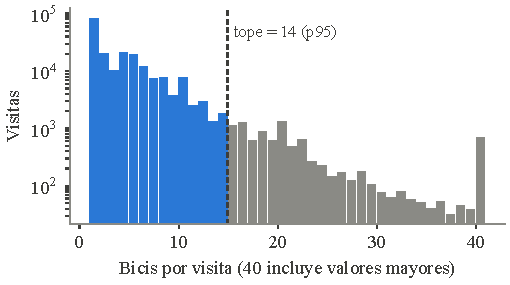
\includegraphics[width=\columnwidth]{figs/tamanos-run3.pdf}
\caption{Bicis por visita de Ecobici, \rfigPeriodo{} (\rfigVisitas{} visitas, sin pares). En azul, hasta el tope de \rtopeBicis{}: el \rfigBajoTope\% de las visitas. Escala logarítmica.}
\label{fig:tamano}
\end{figure}

\begin{figure}[t]
\centering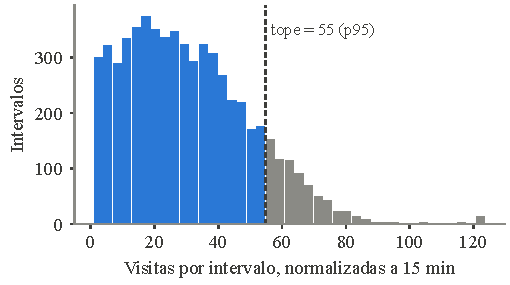
\includegraphics[width=\columnwidth]{figs/visitas-tope-run3.pdf}
\caption{Visitas de Ecobici por intervalo entre fotos, llevadas a 15 minutos (visitas $\times$ 15 / minutos del intervalo), \rfigPeriodo{} (\rfigIntervalos{} intervalos). En azul, hasta el tope de \rtopeVis{}: el \rfigVisBajoTope\% de los intervalos.}
\label{fig:tope}
\end{figure}

\textbf{Bodega cerrada.} No entran ni salen bicis del sistema. Cada decisión recoge exactamente las bicis que entrega, y la camioneta termina el día vacía. Es coherente con lo que se observa: el total de bicis ancladas a las 04:45 no crece de forma sostenida de un día a otro.

\textbf{Pares que se deshacen.} El feed y los viajes no están sincronizados al segundo. Si una bici sale segundos antes de la foto, la foto todavía la muestra y la ecuación~\eqref{eq:delta} da $+1$; en el intervalo siguiente da $-1$. Un movimiento que se deshace exacto en el intervalo inmediato, en la misma estación, no se cuenta como visita. La regla se aplica igual a nuestras órdenes.

% ======================================================================
\section{Resultados y discusión}\label{sec:resultados}
Primero describimos las cinco piezas del método: qué recibe cada una, qué entrega y por qué la elegimos. Al final van los resultados.

\subsection{Simulador}
\textbf{Entra:} el estado de cada estación a las 05:00, los viajes del día, los cambios de etiqueta observados y las órdenes de una política. \textbf{Sale:} las bicis disponibles de cada estación en cada minuto, $E$, $F$, visitas, bicis movidas y desvíos.

El simulador procesa eventos en orden de tiempo. Cuando varios caen en el mismo instante, el orden es: cambios de etiqueta, recogidas y entregas, decisión de la política, llegadas de viajes y salidas. Al inicio de cada minuto, después de los eventos de ese instante, toma una muestra de cada estación. Cuenta un minuto en $E$ si la estación tiene 0 disponibles y en $F$ si disponibles, no rentables y anclajes fuera de servicio llenan la capacidad.

La Tabla~\ref{tab:linea} muestra la vida de una orden. Al recoger, se toma lo pedido hasta el tope por visita y hasta lo que haya. Al entregar, se reparte la carga real entre los destinos; si falta carga, el recorte es proporcional. Si un destino ya no tiene espacio, el sobrante regresa a la estación con espacio más cercana al origen. Ninguna bici se crea ni se pierde: una verificación de conservación corre después de cada evento.

\begin{table}[t]
\centering\footnotesize
\caption{Vida de una decisión emitida a las 08:00.}
\label{tab:linea}
\begin{tabularx}{\columnwidth}{@{}lY@{}}
\toprule
Hora & Qué pasa \\
\midrule
08:00 & el asignador lee el estado y sus órdenes pendientes y emite recogidas y entregas que suman lo mismo \\
08:00--08:15 & siguen los viajes; las estaciones cambian \\
08:15 & recogida: se toman las bicis que haya, hasta \rtopeBicis{} por visita \\
08:15--09:00 & las bicis van en la camioneta; siguen los viajes \\
09:00 & entrega: se reparte la carga; el sobrante vuelve cerca del origen \\
\bottomrule
\end{tabularx}
\end{table}

El rebalanceo de Ecobici se reproduce así: cada movimiento $\delta_i$ se aplica en la hora $t_1$ de la foto, limitado por lo que físicamente cabe. Como son movimientos medidos, su neto no tiene que ser cero (ver amenazas).

\subsection{Pronósticos}
\textbf{Sale:} salidas y llegadas esperadas por estación y por cuarto de hora para las próximas $n$ horas. Hay dos formas. La \emph{diaria} se calcula una vez a las 05:00 para todo el día, por hora de reloj. La \emph{directa} se recalcula cada \rstepMin{} minutos para las siguientes horas móviles, usando lo observado ese día. Ambas reparten cada hora en partes iguales entre sus cuatro cuartos.

\textbf{Media móvil (diaria).} Para cada estación y hora de reloj, promedia los conteos de los días del mismo tipo (entre semana, o fin de semana y festivo) en las \rsemanasHist{} semanas previas. No se entrena nada. Es la referencia más simple que usa la estacionalidad semanal.

\textbf{LightGBM diario.} Dos modelos de árboles con potenciación de gradiente \cite{ke2017lightgbm}, uno para salidas y otro para llegadas, con pérdida Poisson porque el objetivo es un conteo. Cada fila es una estación en una hora del día. Variables: estación (categórica), minuto de inicio de la hora, día de la semana, festivo, \texttt{lag7} y \texttt{lag14} (el conteo de esa hora hace 7 y 14 días) y \texttt{mean28} (la media de los días del mismo tipo en \rsemanasHist{} semanas). Parámetros fijos, sin búsqueda: \rlgbArboles{} árboles, tasa \rlgbTasa, \rlgbHojas{} hojas, al menos \rlgbMinHoja{} filas por hoja, \rlgbFilas{} de las filas y \rlgbCols{} de las variables por árbol. Se elige porque capta interacciones entre estación, hora y día sin especificarlas a mano.

\textbf{LightGBM directo.} El mismo modelo con cuatro variables más: \texttt{k} (cuántas horas adelante), \texttt{last15} y \texttt{last60} (salidas o llegadas de la estación en el último cuarto y en la última hora) y \texttt{elapsed\_delta} (lo acumulado en el día menos lo acumulado en un día típico a esa hora). Esas variables del día salen de los viajes registrados de ese mismo día, solo con viajes ya terminados antes de $t$. Para entrenar se usa uno de cada \rcadaTicks{} instantes de decisión por día, con una fase que rota para cubrir todas las horas.

\textbf{Entrenamiento.} Para cada mes de prueba, los modelos se entrenan con los \rtrainMeses{} meses anteriores, nunca con días posteriores. Cada día de entrenamiento necesita sus \rsemanasHist{} semanas previas completas.

\textbf{Oráculos.} Reciben los conteos reales del día: el diario, por hora de reloj; el directo, por hora móvil desde $t$. Conocen los totales, no el minuto de cada viaje. No son una estrategia posible. Sirven de techo: dicen cuánto lograría el mismo asignador con información perfecta a esa resolución. Tampoco son el óptimo matemático, porque el asignador sigue teniendo topes y tiempos.

\subsection{Asignador}
\textbf{Entra:} en el minuto $t$, el estado de las estaciones, las órdenes pendientes, el pronóstico y dos parámetros, $n$ (horas de pronóstico que mira) y $\lambda$ (precio de una visita en minutos-estación de $\EF$). \textbf{Sale:} cuántas bicis recoger o entregar en cada estación.

\textbf{Proyección.} El pronóstico se convierte en un flujo neto por minuto, $f_{im}=(\text{llegadas}-\text{salidas})/15$ dentro de cada cuarto. Con ese flujo, más las órdenes pendientes en su hora, proyectamos el inventario de cada estación minuto a minuto, recortado a $[0,K_i]$, donde $K_i$ son los lugares para bicis disponibles. Así obtenemos $p_i$, el inventario proyectado a $t+\rpickMin$, y $q_i$, el proyectado a $t+\rdelMin$. De ahí salen los máximos $r_i=\min(B,\lfloor p_i\rfloor)$ para recoger y $u_i=\min(B,\lfloor K_i-q_i\rfloor)$ para entregar, con $B=\rtopeBicis$.

\textbf{Costo por estación.} Para cada cantidad posible, $c^R_i(x)$ es el cambio en minutos de $E$ o $F$ de la estación $i$ entre $t+\rpickMin$ y $t+60n$ si se recogen $x$ bicis en $t+\rpickMin$, frente a no hacer nada. $c^E_i(x)$ es lo mismo para entregar $x$ bicis en $t+\rdelMin$. Ambos se calculan con la proyección minuto a minuto. Como $c$ no es convexo, usamos su envolvente convexa inferior, que es lineal por tramos. Cada tramo $k$ tiene pendiente $\alpha_{ik}$ y ordenada $\beta_{ik}$.

\textbf{Programa entero.} Variables: $x^R_i, x^E_i$ enteras (bicis a recoger y entregar), $y^R_i, y^E_i$ binarias (si hay visita) y $z^R_i, z^E_i$ continuas (costo de cada pierna).
\begin{align}
\min\ & \textstyle\sum_i (z^R_i+z^E_i)+\lambda\sum_i (y^R_i+y^E_i) \label{eq:obj}\\
\text{s.a.}\ & x^R_i\le r_i\,y^R_i,\quad x^E_i\le u_i\,y^E_i \label{eq:c1}\\
& y^R_i+y^E_i\le 1 \label{eq:c2}\\
& z^R_i\ge \alpha^R_{ik}x^R_i+\beta^R_{ik}y^R_i\quad\forall k \label{eq:c3}\\
& z^E_i\ge \alpha^E_{ik}x^E_i+\beta^E_{ik}y^E_i\quad\forall k \label{eq:c4}\\
& \textstyle\sum_i x^R_i=\sum_i x^E_i \label{eq:c5}\\
& \textstyle\sum_i (y^R_i+y^E_i)\le V \label{eq:c6}
\end{align}
La función objetivo~\eqref{eq:obj} suma los minutos de $\EF$ que cambian y cobra $\lambda$ por visita. \eqref{eq:c1}: solo se mueven bicis si hay visita, y no más de lo que hay o cabe. \eqref{eq:c2}: una estación no recoge y entrega en la misma decisión. \eqref{eq:c3}--\eqref{eq:c4}: el costo de cada pierna sigue la envolvente; sin visita, el costo es cero. \eqref{eq:c5}: bodega cerrada, se entrega lo que se recoge. \eqref{eq:c6}: a lo más $V=\rtopeVis$ visitas por decisión.

\textbf{Qué son $n$ y $\lambda$.} Con $n=1$ el asignador no hace nada, porque la entrega cae justo al final de su horizonte. Con $n$ mayor ve más consecuencias, pero con pronósticos más inciertos. Una visita solo vale la pena si ahorra más de $\lambda$ minutos-estación; un $\lambda$ alto da menos visitas.

\textbf{Resolución.} El programa lo resuelve HiGHS, un resolvedor de código abierto de programación lineal y entera \cite{huangfu2018highs}, con brecha relativa de $10^{\rbrechaExp}$ y un límite de \rlimiteS~s por decisión. Si llega al límite con una solución factible, la usa. Solo si no tiene ninguna, o si la solución viola alguna restricción, esa decisión no emite órdenes. En la prueba hubo \rdecTot{} decisiones; \rdecLim{} llegaron al límite y \rdecFallback{} quedaron sin solución. Elegimos un programa entero, y no una regla de umbrales por estación, porque reparte un cupo común de visitas y obliga a que lo recogido sea lo entregado. La envolvente convexa es una aproximación: en un caso sintético con flujo aleatorio, el orden que da a planes alternativos coincide con el $\EF$ simulado (Spearman mediano \rspearman).

\subsection{Medición de Ecobici}
Aplicamos la ecuación~\eqref{eq:delta} a cada par de fotos consecutivas de cada estación, con la hora corregida \rlagS{} s. Un $\delta_i\ne0$ es una visita de Ecobici. Después quitamos los pares que se deshacen. En los \rrefDias{} días de referencia, sin la regla Ecobici tendría \rvisSinRegla{} visitas por día; con ella, \rvisConRegla{} (el \rvisQuedan\%). La regla le baja el esfuerzo medido a Ecobici, así que nos pone una vara más alta. El Apéndice~\ref{ap:auditoria} da la tabla completa y ejemplos reales. La medición tiene un límite: si en un intervalo traen una bici y se llevan tres, vemos $-2$. Lo medido es un piso del esfuerzo real.

\subsection{Diseño de la prueba}
\textbf{Selección.} \rselDias{} días de \rselMes{} (\rselLab{} entre semana y \rselFin{} de fin de semana, sorteados con semilla fija). Con los dos oráculos y $\lambda\in\{\rlamGridN\}$ probamos $n$ de 1 a \rnMax{} horas. Nos quedamos con el primer $n$ cuyo siguiente no mejora de forma significativa (IC95 pareado por día): $n=\rnDiario$ en ambas formas. Después, para cada brazo, buscamos el $\lambda$ con el que hace tantas visitas como Ecobici en esos días (\rselEcoVis{} por día). Para la media móvil, $\lambda=\rlamMa$ da \rselMaVis{} visitas. En \rlamExtrap{} brazos (media móvil y los dos LightGBM) ese $\lambda$ quedó por encima de la rejilla; se extrapoló y se confirmó con otra corrida.

\textbf{Prueba.} Todos los días de \rpruebaPeriodo{} con al menos \rcovMin\% de sus horas cubiertas por fotos: \rdias{} días. Nada se ajustó con ellos. Los modelos de cada mes se entrenan con los \rtrainMeses{} meses anteriores. Las diferencias se reportan con IC95 $t$ pareado por día.

\subsection{Resultados}
La Tabla~\ref{tab:brazos} resume los siete brazos y la Tabla~\ref{tab:principal} los resultados. Sin rebalanceo, el sistema acumula \rbaseEF{} minutos-estación de $\EF$ por día. El rebalanceo medido de Ecobici lo baja a \recoEF. La media móvil con el asignador llega a \rmaEF: \rmaPct\% menos que Ecobici (IC95 \rmaPctLo--\rmaPctHi\%), con menos tiempo vacío y mucho menos tiempo lleno (\rmaE{} y \rmaF{} minutos-estación). Gana en \rmaGana{} de \rdias{} días. Hizo \rmaVis{} visitas y movió \rmaBicis{} bicis por día, contra \recoVis{} y \recoBicis{} de Ecobici. La Fig.~\ref{fig:ef} muestra lo mismo.

\begin{table}[t]
\centering\footnotesize
\caption{Brazos comparados. Los cinco con asignador usan $n=\rnDiario$ horas.}
\label{tab:brazos}
\begin{tabular}{@{}llr@{}}
\toprule
Brazo & Qué decide las órdenes & $\lambda$ \\
\midrule
Sin rebalanceo & nada; solo viajes y etiquetas & --- \\
Ecobici (medido) & movimientos inferidos del feed & --- \\
Media móvil & asignador + media de 4 semanas & 58.2 \\
LightGBM diario & asignador + LightGBM a las 05:00 & 59.2 \\
LightGBM directo & asignador + LightGBM cada 15 min & 68.9 \\
Oráculo diario & asignador + viajes reales por hora & 44.6 \\
Oráculo directo & asignador + viajes reales, hora móvil & 36.3 \\
\bottomrule
\end{tabular}

\end{table}

\begin{table}[t]
\centering\footnotesize
\setlength{\tabcolsep}{4pt}
\caption{Medias por día en \rdias{} días de prueba. E+F en minutos-estación. La última columna es la reducción frente a Ecobici, con IC95 $t$ pareado por día.}
\label{tab:principal}
\begin{tabular}{@{}lrrrr@{}}
\toprule
Brazo & E+F & Visitas & Bicis & Menos E+F, \% \\
\midrule
Sin rebalanceo & 217,943 & 0 & 0 & --- \\
Ecobici (medido) & 100,641 & 2,236 & 10,217 & --- \\
Media móvil & 56,542 & 2,000 & 8,670 & 43.8 [41.7, 46.0] \\
LightGBM diario & 57,026 & 2,000 & 8,342 & 43.3 [41.2, 45.5] \\
LightGBM directo & 56,588 & 1,992 & 9,238 & 43.8 [41.7, 45.8] \\
\midrule
Oráculo diario & 37,162 & 1,958 & 8,600 & 63.1 [60.6, 65.5] \\
Oráculo directo & 28,897 & 1,968 & 7,905 & 71.3 [68.3, 74.3] \\
\bottomrule
\end{tabular}

\end{table}

\begin{figure}[t]
\centering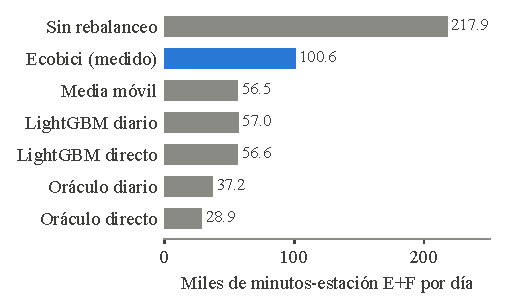
\includegraphics[width=\columnwidth]{figs/ef-brazos-run3.pdf}
\caption{$\EF$ medio por día en los \rdias{} días de prueba. En azul, el rebalanceo medido de Ecobici.}
\label{fig:ef}
\end{figure}

Los tres pronósticos reales empatan. LightGBM diario (\rlgbmDPct\%) y LightGBM directo (\rlgbmDirPct\%) no superan a la media móvil. Su exactitud tampoco es mejor (Apéndice~\ref{ap:pron}). La ventaja viene de asignar con un pronóstico razonable; un modelo más complejo no agregó nada. La mejora se sostiene en el tiempo: \rdicPct\% en \rdicMes{} y \renePct\% en \reneMes.

\textbf{Oráculos.} Con los viajes reales, el mismo asignador llega a \rorDEF{} (diario) y \rorDirEF{} (directo). Entre la media móvil y su oráculo hay \rmaGap{} minutos-estación por día: es lo que cuesta no conocer el futuro. El oráculo directo deja \roracleDirectGap{} minutos-estación menos que el diario: con información perfecta, actualizar cada \rstepMin{} minutos sí vale. Con LightGBM directo esa ventaja no aparece; su brecha contra su oráculo es \rlgbmDirGap.

\subsection{Interpretación y amenazas}
\textbf{Esfuerzo.} El $\lambda$ se fijó para igualar las visitas de Ecobici en \rselMes. En la prueba la media móvil hizo \rmaVisPct\% menos visitas. La comparación no es a igual esfuerzo exacto, pero el error favorece a Ecobici.

\textbf{El rebalanceo de Ecobici no cierra en cero.} Al reproducirlo, su neto suma \recoNeto{} bicis por día dentro de la ventana; nuestras políticas no reciben bicis de fuera. Esta asimetría también favorece a Ecobici.

\textbf{La medición es un piso.} Solo vemos netos entre fotos; si Ecobici trae y se lleva en el mismo intervalo, no lo vemos. Su esfuerzo real puede ser mayor. Al reproducir sus movimientos, el simulador da un $E$ \rvRel\% menor y un $F$ \rvRelF\% menor que los observados en las fotos (Apéndice~\ref{ap:auditoria}).

\textbf{Logística.} Los topes limitan visitas y bicis, no rutas. No sabemos si una flota real puede ejecutar cada decisión. El tiempo de entrega es el supuesto más sensible.

\textbf{Demanda.} Los viajes son los registrados. Con menos estaciones vacías habría viajes nuevos que no están en los datos, y con desvíos algunos viajes reales no ocurrirían. Por eso no traducimos los minutos ahorrados a viajes.

% ======================================================================
\section{Conclusiones}
\textbf{Recomendación.} En simulación, asignar cada \rstepMin{} minutos con un pronóstico sencillo deja \rmaPct\% menos minutos vacíos o llenos que el rebalanceo actual de Ecobici, con menos visitas, en todos los días de prueba. Recomendamos a Ecobici y a SEMOVI un piloto en una microzona con demanda alta, como Buenavista--Reforma, comparando contra una zona parecida sin cambios. La herramienta mínima es la media móvil más el asignador: no necesita entrenar modelos, y en la prueba el percentil 95 diario del tiempo por decisión nunca pasó de \rdecPNoventaCinco{} s.

\textbf{Implementación.} El piloto necesita registrar cada orden, la camioneta que la hizo, la hora de recogida y de entrega, y las bicis cargadas. Con eso se calibran los \rpickMin{} y \rtransMin{} minutos, los topes y $\lambda$. Los riesgos son tres: que las rutas no permitan cumplir las órdenes a tiempo, que el tráfico alargue los traslados y que los usuarios no se desvíen como supone el simulador. Si los tiempos reales fueran mucho mayores, la ventaja bajaría (Apéndice~\ref{ap:sens}). Para usar LightGBM directo, el operador necesita las salidas y llegadas del día en vivo. Ecobici probablemente las tiene; si no, las puede separar de sus propios movimientos, porque sabe qué cambios de inventario son de sus camionetas.

\textbf{Trabajo futuro.} (1) Añadir rutas y número de vehículos al asignador. (2) Estimar la demanda no atendida para pasar de minutos a viajes. (3) Usar el registro de órdenes del piloto para validar la medición de Ecobici. (4) Explorar por qué el pronóstico directo no aprovecha la información del día, que con el oráculo sí vale \roracleDirectGap{} minutos-estación por día.

\clearpage
\sloppy
\bibliographystyle{IEEEtranN}
\bibliography{referencias}

\clearpage
\appendices
\section{Auditoría de movimientos y pares}\label{ap:auditoria}
\textbf{Pares.} La Tabla~\ref{tab:pares} muestra cuántas visitas de Ecobici quedan según el tamaño de los pares que se quitan, en los \rrefDias{} días de referencia (05:00 a 00:30). ``Entran'' y ``Salen'' son bicis por día.

\begin{table}[h]
\centering\footnotesize
\setlength{\tabcolsep}{4pt}
\caption{Efecto de quitar pares que se deshacen. Media por día.}
\label{tab:pares}
\begin{tabular}{@{}lrrrr@{}}
\toprule
Regla & Visitas & Entran & Salen & Visitas que quedan, \% \\
\midrule
Sin regla & 5,113.5 & 7,042.9 & 7,059.1 & 100.0 \\
Solo $\pm1$ & 2,722.9 & 5,847.6 & 5,863.8 & 53.2 \\
Hasta $\pm2$ & 2,542.9 & 5,667.6 & 5,683.8 & 49.7 \\
Hasta $\pm3$ & 2,513.3 & 5,623.2 & 5,639.4 & 49.1 \\
Cualquier tamaño & 2,491.5 & 5,568.4 & 5,584.6 & 48.7 \\
\bottomrule
\end{tabular}

\end{table}

Ejemplo real: estación 002, 3 de septiembre de 2025. Entre las fotos de 11:48:28 y 12:08:14 la ecuación~\eqref{eq:delta} da $+1$; entre 12:08:14 y 12:25:18 da $-1$. La bici 4201141 salió de esa estación a las 12:07:09, segundos antes de la foto. La foto todavía la mostraba anclada; en la siguiente ya no estaba. No hubo camioneta. Los pares casi no aparecen en intervalos sin viajes y crecen con el número de viajes, como se espera de un desfase de relojes.

En \rcurvaDias{} días de sensibilidad, sin la regla Ecobici sumaría \rsSinRegla{} visitas por día; quitando solo los pares de una bici, \rsSoloUno. Su $\EF$ no cambia (\rsEcoEF): un par suma cero.

\textbf{Validación del simulador.} En los \rrefDias{} días de referencia, las fotos muestran \rvEobs{} minutos-estación vacíos y \rvFobs{} llenos por día. Al reproducir los movimientos de Ecobici, el simulador da \rvErep{} y \rvFrep. La diferencia viene de los desvíos, los pares, los cambios de etiqueta que no se pueden aplicar y de que el feed se ve en escalones mientras el simulador aplica cada viaje a su segundo.

\section{Sensibilidades}\label{ap:sens}
En \rcurvaDias{} días, contra el caso base de la media móvil (diferencia en $\EF$ por día, IC95): entregar a los \rentregaCorta{} minutos, \rsCuarenta{} [\rsCuarentaLo, \rsCuarentaHi]; a los \rentregaLarga, \rsSetenta{} [\rsSetentaLo, \rsSetentaHi]. Topes del percentil 99 (\rtopeVisNN{} visitas, \rtopeBicisNN{} bicis), \rsNN{} [\rsNNLo, \rsNNHi]. Topes medidos de \rantPeriodo{} (\rtopeVisAnt{} y \rtopeBicisAnt), \rsAnt{} [\rsAntLo, \rsAntHi]. No rentables que siguen el feed tal cual (llegan o se van con el total), \rsDan{} [\rsDanLo, \rsDanHi]. Para el oráculo directo: \rsCuarentaOr, \rsSetentaOr, \rsNNOr, \rsAntOr{} y \rsDanOr. El tiempo de entrega pesa más que los topes.

\section{Exactitud del pronóstico}\label{ap:pron}
Error absoluto medio del neto (llegadas menos salidas) por estación y hora, primera hora, \rmaeMes: media móvil \rmaeMa, LightGBM diario \rmaeLgbmD, LightGBM directo \rmaeLgbmDir. El WAPE es \rmaeMaW, \rmaeLgbmDW{} y \rmaeLgbmDirW. Los oráculos tienen error cero en sus propios bloques. Un error chico en una estación crítica puede costar más $\EF$ que varios en una estación holgada; por eso comparamos pronósticos por su $\EF$ y no solo por su error.

\section{Cómo reproducir}\label{ap:repro}
Código: \cite{repo}. Todos los comandos se corren con \texttt{uv run} desde la raíz.

\begin{center}\footnotesize
\begin{tabularx}{\columnwidth}{@{}p{2.7cm}Y@{}}
\toprule
Qué & Comando (\texttt{uv run} \dots) \\
\midrule
Viajes y fotos & \texttt{python -m ecosim.data build-trips} y \texttt{build-snapshots} \\
Movimientos de Ecobici, topes, Tabla~\ref{tab:pares} & \texttt{python -m ecosim.medicion} \\
Pronósticos y exactitud & \texttt{python -m ecosim.pronostico} \\
Experimento, Tablas~\ref{tab:brazos}--\ref{tab:principal} & \texttt{python -m ecosim.run -{}-all} \\
Validación del asignador & \texttt{python -m ecosim.asignador validate} \\
Cifras, tablas, Figs.~\ref{fig:tamano}--\ref{fig:ef} & \texttt{python3 report/figs/numeros\_run3.py} \\
Comprobar cifras & el mismo, con \texttt{-{}-check} \\
\bottomrule
\end{tabularx}
\end{center}
Cada cifra del texto es una macro con su origen en \texttt{report/fuentes-numeros.md}.
\end{document}
